\subsection{W-DCGAN}
\label{sec:exp-w-dcgan}
We present the evolution of the inception score and losses in Figures \ref{fig:exp-w-dcgan-is} and \ref{fig:exp-w-dcgan-losses}, respectively.
   
\begin{figure}[t!]
    \centering
    \begin{subfigure}[t]{0.49\textwidth}
        \centering
		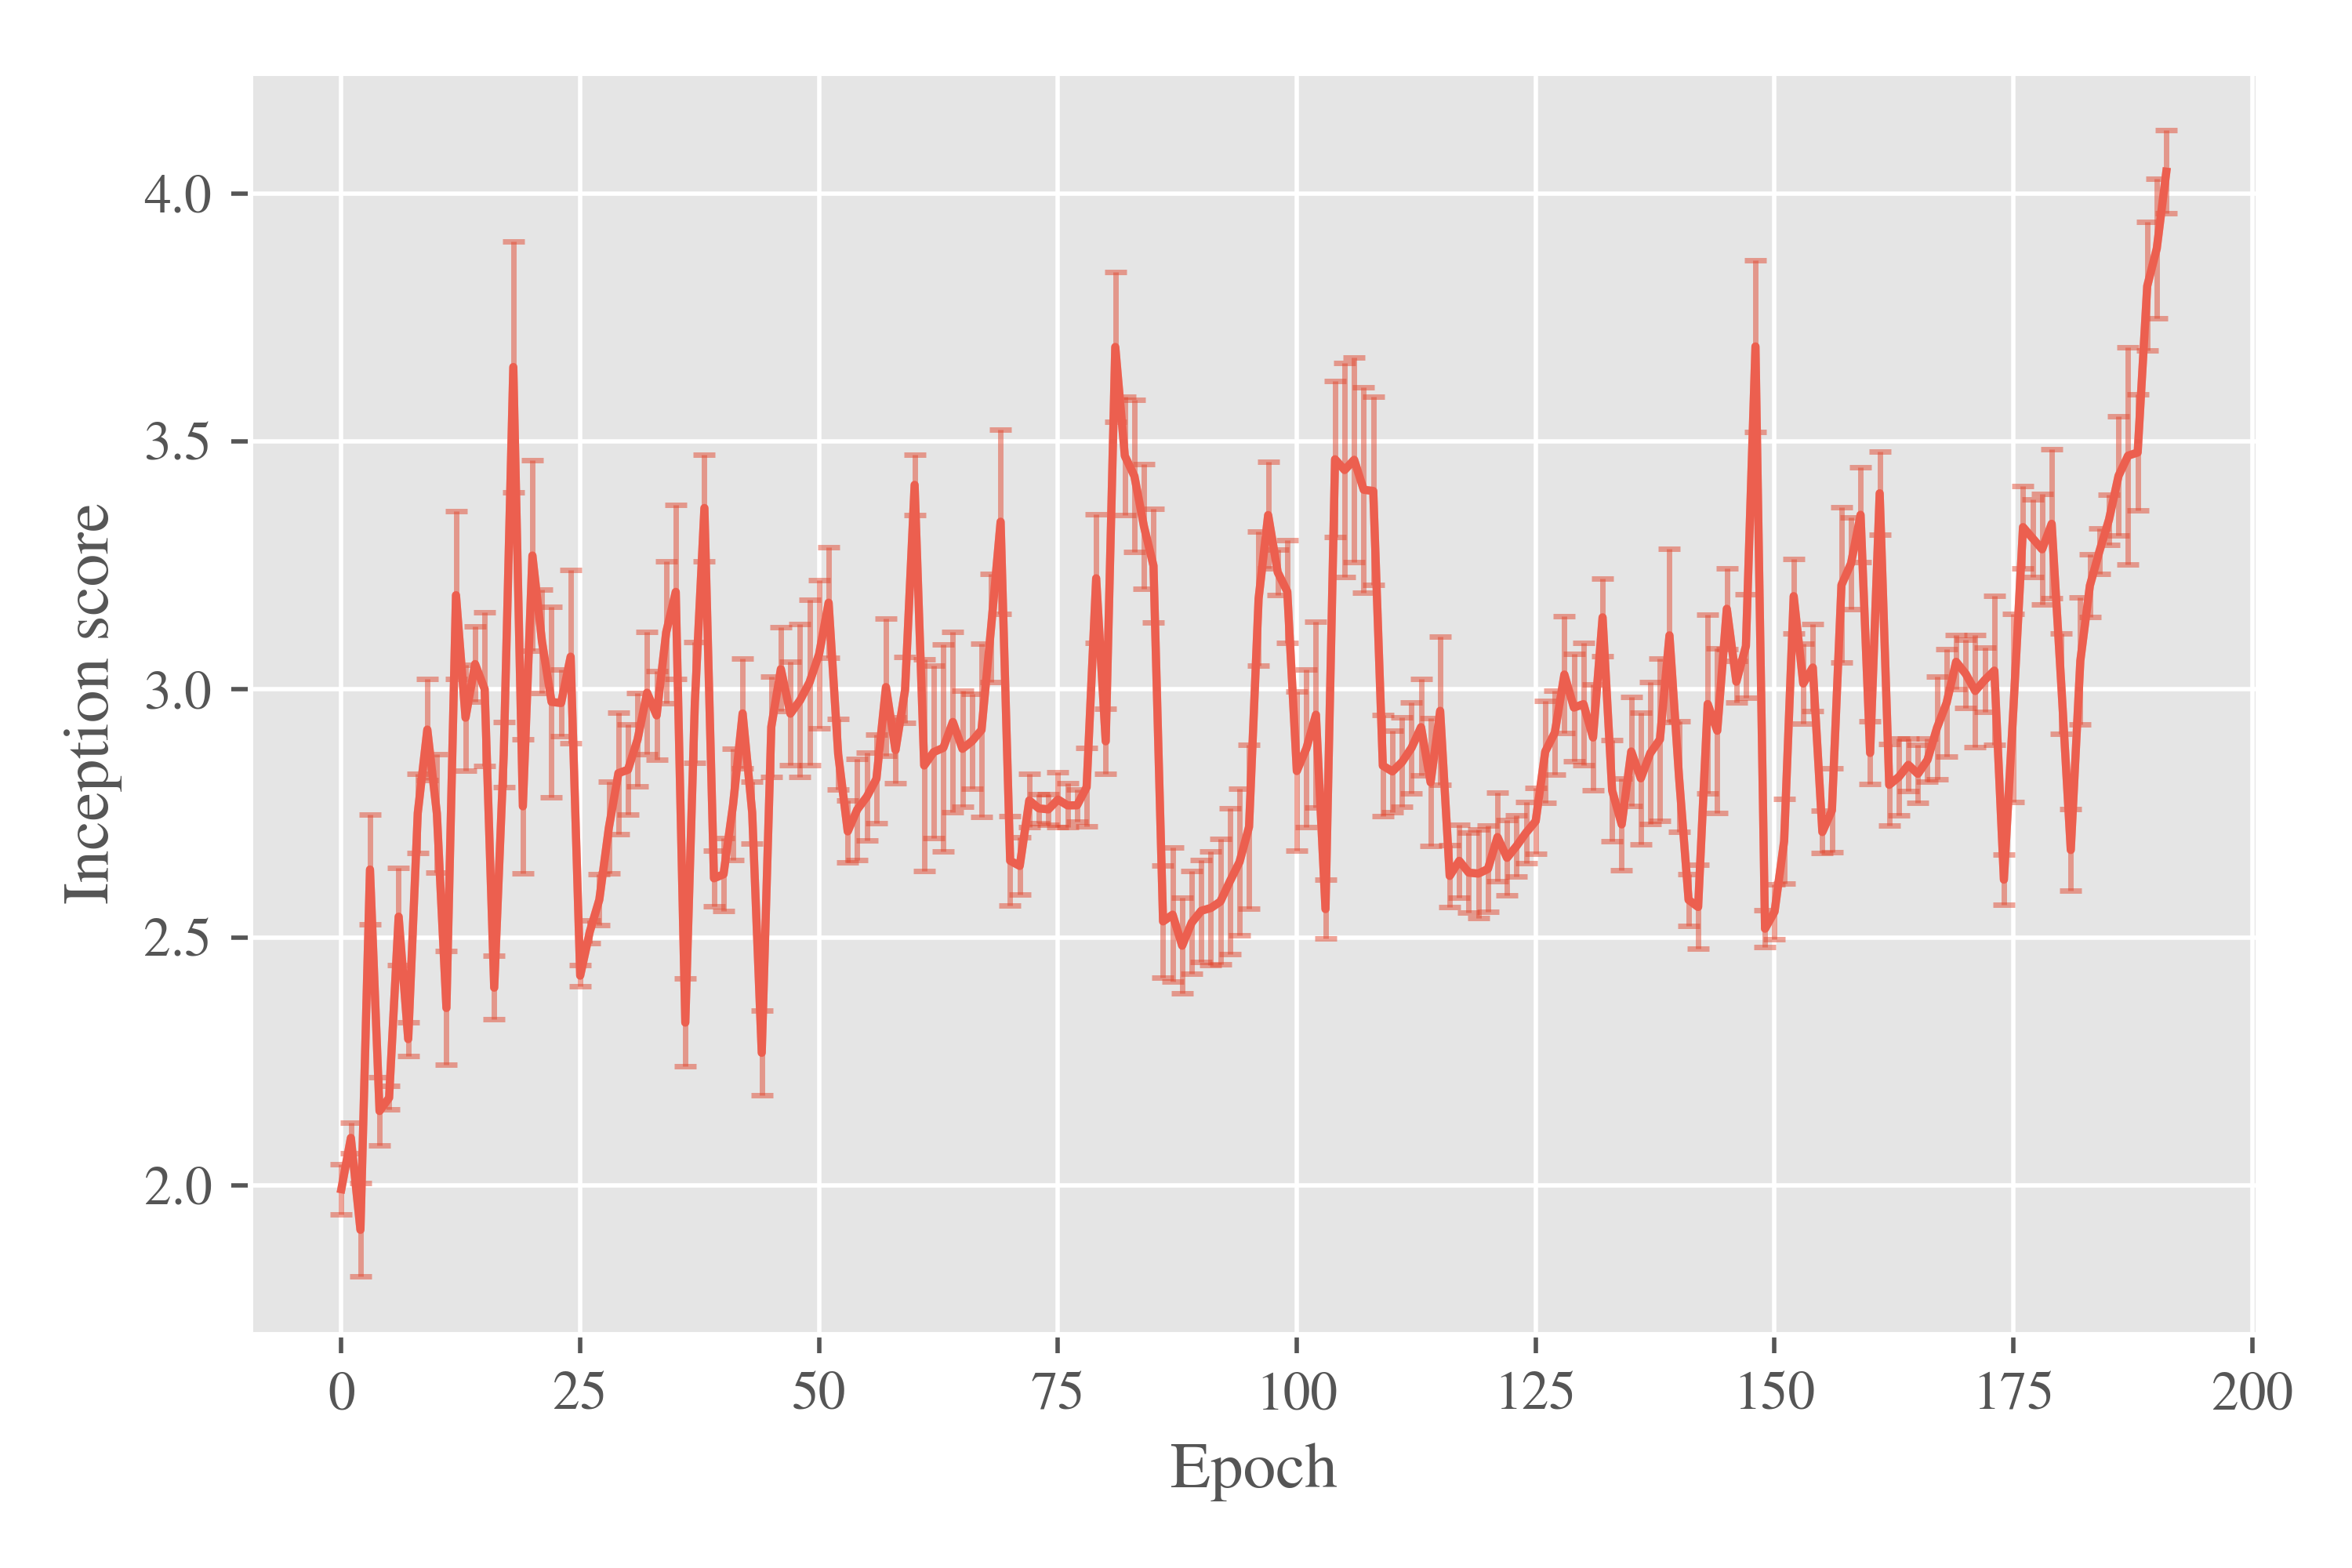
\includegraphics[width=\textwidth]{../code/results/figures/w-dcgan_cifar10_is.png}
		\caption{Inception score}
		\label{fig:exp-w-dcgan-is}
    \end{subfigure}
    \begin{subfigure}[t]{0.49\textwidth}
        \centering
        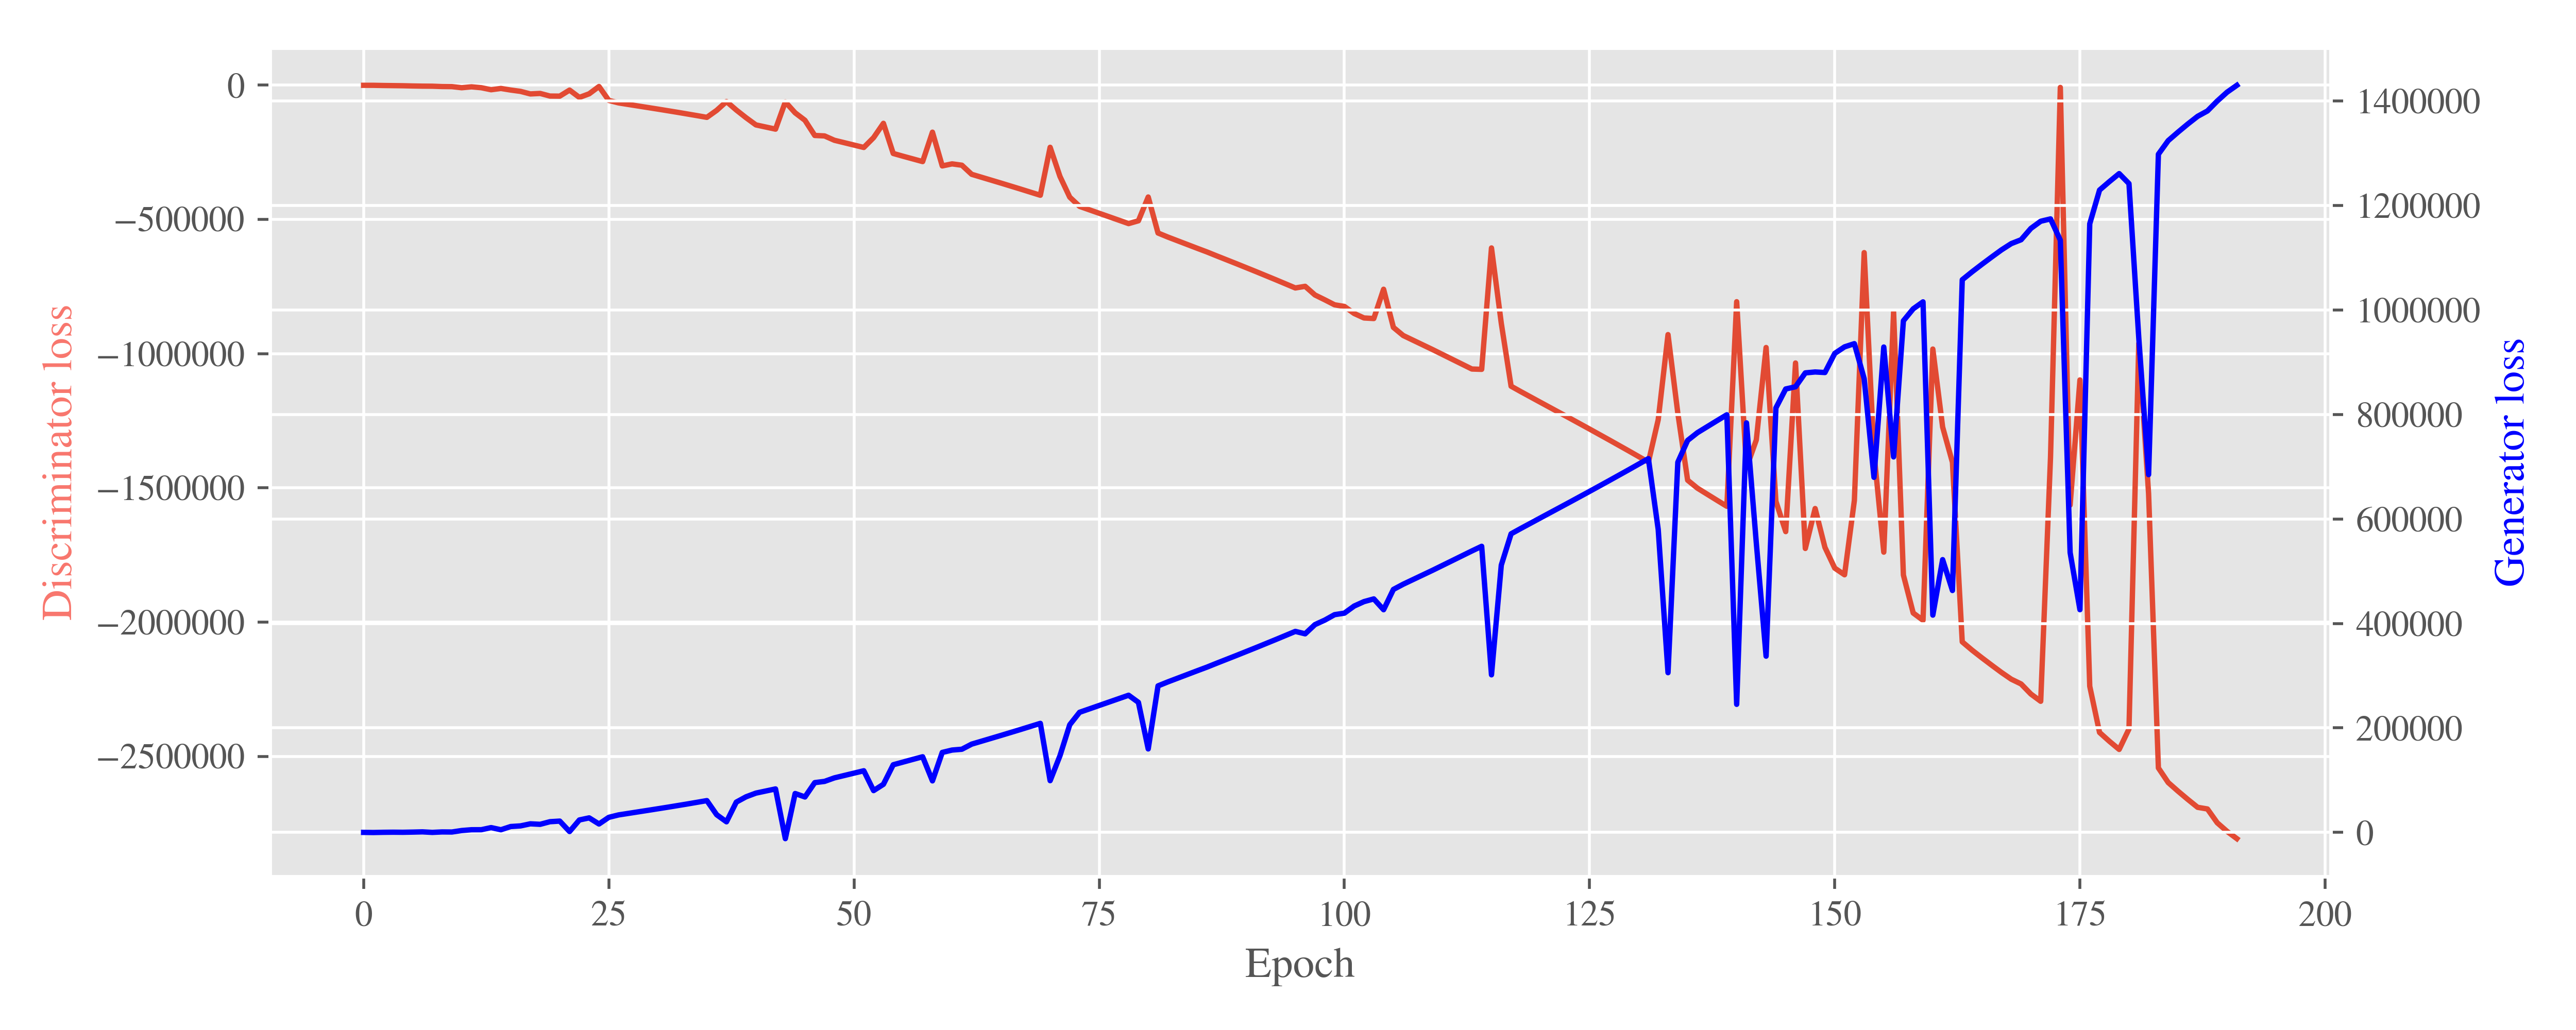
\includegraphics[width=\textwidth]{../code/results/figures/w-dcgan_cifar10_losses.png}
		\caption{Losses}
		\label{fig:exp-w-dcgan-losses}
    \end{subfigure}
    \caption{W-DCGAN - training on CIFAR10 over 200 epochs.}
\end{figure}